%make it clear that students should plot on log-log graph
\documentclass[11pt,letterpaper]{article}
\usepackage{array}
\usepackage{fullpage}
\usepackage{graphicx}
\usepackage{parskip}
\usepackage{amsmath}
\usepackage[small]{caption}
\usepackage{graphpap}
\usepackage{logpap}
\usepackage{tabularx}
\usepackage{url}
\usepackage{hyperref}
\usepackage{enumitem}

\renewcommand{\thesection}{PART \arabic{section}: }

\newcounter{question}[section]
\newenvironment{question}[1][]{\refstepcounter{question}\par\medskip
   \textbf{\arabic{section}.\thequestion.} \rmfamily}{\medskip}

\usepackage{titlesec}
\titleformat{\section}{\clearpage\normalfont\bfseries}{\thesection}{0em}{}
\titlespacing{\section}{0pt}{0.5\baselineskip}{0pt}

\titleformat{\subsection}[runin]
{\normalfont\bfseries}{\thesubsection}{1em}{}

\titleformat{\subsubsection}{\normalfont\bfseries}{\thesubsubsection}{0em}{}
\titlespacing{\subsubsection}{0pt}{0.5\baselineskip}{0pt}

\newcounter{saveenumi}
\newcommand{\seti}{\setcounter{saveenumi}{\value{enumi}}}
\newcommand{\conti}{\setcounter{enumi}{\value{saveenumi}}}

\usepackage[dvipsnames]{xcolor}
\newcommand{\sol}[1]{{\color{NavyBlue} #1}}


\begin{document}
\setlength{\parindent}{0in}

%% EQUIP: Force Probe, Pulley, Track, Hangar, Weight, Tilt, Scale

\begin{flushright}
PHYS S211: General Physics I\\ 
Lab 9: Pendulums and Resonance\\
11/22/22 (due 12/2/22)
\end{flushright}

Name(s):\\

\subsubsection*{Topics:}
\begin{enumerate}
\setlength{\parskip}{3pt}
\item Period of a pendulum
\item Pendulum speed
\item Resonance
\end{enumerate}
 
\subsubsection*{Introduction:}
Until the industrial revolution, interest in the measurement of time was almost entirely concentrated on the construction of calendars for agricultural purposes.  Although the Egyptians were the first to divide day and night into 12 hours each, there was no technology for measuring time units smaller than a day with great accuracy until four thousand years later.

Galileo was the first to realize that a pendulum could be used to measure time accurately --- previously, he had been using his own pulse to measure the time required for objects
to roll down inclined planes.  Legend has it that the idea came to him while he watched a chandelier swinging during a church service.  Sentenced to house arrest for suspicion of
heresy, he spent the last years of his life trying to build a more practical pendulum clock that would run for long periods of time.  This technical feat was only achieved later by Christian Huygens.  Along with the Chinese invention of the compass, accurate clocks were vital for European exploration by sea, because longitude can only be determined by astronomical observations combined with accurate measurements of time.

In this lab you will determine what controls the period of a pendulum, investigate the relationship between a pendulum's length and velocity, and gain some intuition for ``resonance''.

\subsubsection*{What you should turn in:} 
You may submit a group report.
\begin{itemize}
\setlength{\parskip}{3pt}
\item Part 1: Three graphs [6 pts] and results of curve fitting, including interpretation of the constants [3 pts]
\item Part 2: Measurements of $v_{\rm{max}}$ and a graph comparing measured to predicted values of $v_{\rm{max}}$ [3 pts]. Derivation of theoretical value of $v_{\rm{max}}$ [3 pts]. Sketches of how you would expect the position, velocity, kinetic energy, and potential energy to vary with time [4 pts].
\item Part 3: Measured resonance frequency and comparison to natural frequency of the pendulum [3 pts]
\end{itemize}

\subsubsection*{Equipment:}
\begin{itemize}
\setlength{\parskip}{3pt}
\item Ring stand and pendulum holder
\item String, mass hanger, and masses
\item LabQuest interface
\item Photogate
\item Cart
\end{itemize}

\section{PERIOD OF A PENDULUM}
The period, $T$, of a pendulum is defined as the time that it takes the pendulum to undergo one (full) oscillation. 

\begin{figure}[h]
\begin{center}
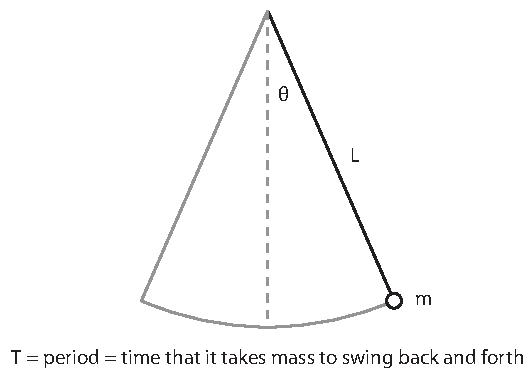
\includegraphics[]{./pendulum}
\end{center}
\end{figure}

In this part of the lab you will explore the relationship between the pendulum's period, the length of the pendulum $L$, the mass of the weight at the end of the pendulum $m$, and the amplitude of the oscillations $\theta_{\rm{max}}$. The amplitude is defined as the maximum angle to which the pendulum rises (i.e., half of the total angle swept out by the pendulum). 

Make several sets of observations to determine how the period, $T$, depends on $\theta_{\rm{max}}$, $L$, and $m$.  As we have done in previous labs, you should use the technique of isolation of variables.  That means that rather than trying many random combinations of $\theta_{\rm{max}}$, $L$, and $m$, you should keep two of them constant while measuring $T$ for various values of the third variable. Then repeat the experiment by varying a different variable and holding the other two constant, and so on. Be sure to try quite a few values of the variable you are changing so that you can clearly see how $T$ depends on each variable. In this experiment it is advantageous to make measurements over a wide range of values because it may be impossible to determine how the period depends on a parameter if you only explore a small range.

You can use a photogate to help you measure the period.

\vspace{.5cm}

Holding $\theta_{\rm{max}}$ constant and $L$ constant.\hspace{1cm} $\theta_{\rm{max}}=$ \hspace{3cm} $L=$

\renewcommand{\arraystretch}{1.4}
\newcolumntype{Y}{>{\centering\arraybackslash}X}
\begin{tabularx}{0.5\linewidth}{|Y|Y|}
\hline
$m$ & $T$ \\
\hline &\\
\hline &\\
\hline &\\
\hline &\\
\hline &\\
\hline
\end{tabularx}\\

\vspace{.5cm}
\clearpage
Holding $m$ and $L$ constant.\hspace{1cm} $m=$ \hspace{3cm} $L=$

\begin{tabularx}{0.5\linewidth}{|Y|Y|Y|}
\hline
$\theta_{\rm{max}}$ & $T$ \\
\hline &\\
\hline &\\
\hline &\\
\hline &\\
\hline &\\
\hline
\end{tabularx}\\

\vspace{.5cm}

Holding $\theta_{\mathrm{max}}$ and $m$ constant.\hspace{1cm} $\theta_{\mathrm{max}}=$ \hspace{3cm} $m=$

\begin{tabularx}{0.5\linewidth}{|Y|Y|}
\hline
$L$ & $T$ \\
\hline &\\
\hline &\\
\hline &\\
\hline &\\
\hline &\\
\hline
\end{tabularx}\\

Graph your data and state your conclusions about whether $T$ depends on $\theta_{\rm{max}}$, $L$ and $m$.  Remember that on a graph of experimental data, the horizontal axis should always be the quantity that you controlled directly (in this case $\theta_{\rm{max}}$, $L$, or $m$) and the vertical axis should be the quantity that you measured but did not directly select (in this case $T$). You should consider (and try to minimize) your sources of error.  There may be some fairly significant systematic errors.
%; for example it is difficult to keep $L$ constant when switching masses.

Of the three variables, find the one on which the period depends most strongly, and use curve fitting techniques to see if you can find a mathematical relationship between the period and that variable. 

HINT: Does this relationship appear linear? What if you plot it on a log-log graph? (Recall that a power law relationship plots as a straight line on a log-log graph.) The equation that you find will have a couple of constants. What is the meaning of the constants? Think about the units to help you figure it out.


%Assume that the equation is of the form 
%\begin{equation}
%T = Cx^p,
%\end{equation}
%where $x$ would actually be $\theta_{\rm{max}}$, $L$, or $m$, and $C$ and $p$ are constants.
%The constant $p$ is important, and is expected to be the same for all pendulums.  For example, if you find that the mass is the variable that has the greatest effect on the period, and that the relationship is of the form $T=Cm^3$, then you have discovered something that is probably generally true for all pendulums: that the period is proportional to the cube of the mass.

IMPORTANT: It may happen that when you change one of the variables, there are only small, insignificant changes in the period, but depending on how you graph the data, it may look like
these are real changes in the period. Most computer graphing software has a default which is to make the $y$-axis stretch only across the range of actual $y$-data. For example if your
periods were all between 0.567 and 0.574 s, then the software makes an extremely magnified graph, with the $y$-axis running only over the short range from 0.567 to 0.574
s. On such a scale, it may seem that there are some major changes in the period even when there are not. To help interpret the graphs, make all of them with the same $y$-scale that goes from zero up to the highest period that you measured. That way you'll be comparing all three graphs on the same footing.



\section{PENDULUM SPEED}
In this part of the lab you will explore the relationship between the maximum speed of a pendulum, $v_{\rm{max}}$, and the length of the pendulum. Set up a photogate to record the horizontal motion of the pendulum as it sweeps through the bottom of its arc. Release the pendulum from some angle $\theta_{\rm{max}}$ and record the maximum velocity. Repeat the experiment three times with different length pendulums, but keep the mass and initial angle constant.

\begin{figure}[h]
\begin{center}
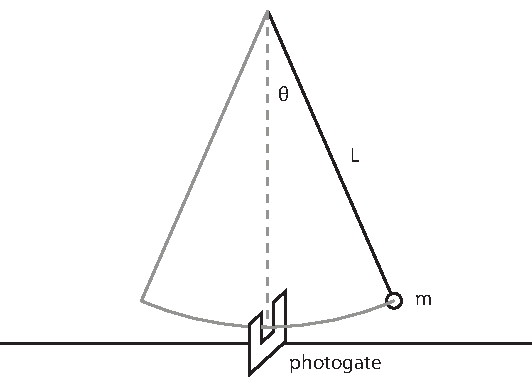
\includegraphics[]{./pendulum_vmax}
\end{center}
\end{figure}

$\theta_{\rm{max}}=$

$m=$

\begin{tabularx}{\linewidth}{|Y|Y|}
\hline
$L$ & $v_{\rm{max}}$ \\
\hline &\\
\hline &\\
\hline &\\
\hline
\end{tabularx}\\

Using kinetic energy and gravitational potential energy, write down an equation for calculating $v_{\rm{max}}$ that depends only on $g$, $L$, and $\theta_{\rm{max}}$. How do your measurements compare to what you would expect from theoretical considerations? Create and submit a plot that compares your measurements to theoretical calculations.
\vspace{4cm}

Based on your observations and derivations, make sketches of how you would expect the angular position, angular speed, kinetic energy, and potential energy of a pendulum to vary with time.

As animals walk they swing their legs back and forth like pendulums. In doing so they let gravity do a lot of work for them. If you assume that an animal's legs can be treated as simple pendulums, what do your results say about the speed with which an animal can comfortably walk (i.e., using the minimum amount of muscle power)?



\section{RESONANCE}
Resonance is a phenomenon that causes a system to experience especially large oscillations. For simple harmonic oscillators that have little damping, such as pendulums, resonance occurs when the system is perturbed with a periodic external forcing that has a frequency close to the natural frequency of the system. The natural frequency is the frequency at which a system will oscillate in the absence of any external forcing.

\begin{figure}[h]
\begin{center}
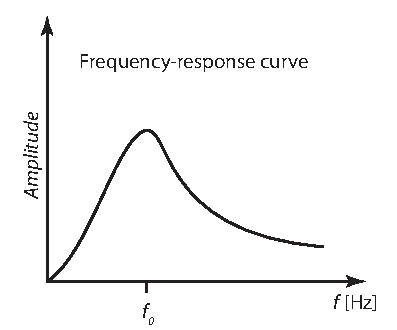
\includegraphics[]{./resonance}
\end{center}
\end{figure}

To test this idea, connect a pendulum to a cart as shown in the diagram below. By moving the cart back and forth with constant amplitude, you will try to determine the natural frequency of the pendulum by determining the driving frequency of the cart that produces the largest oscillations. You should set-up a motion sensor to help you measure the frequency with which you are moving the cart back and forth.

\begin{figure}[h]
\begin{center}
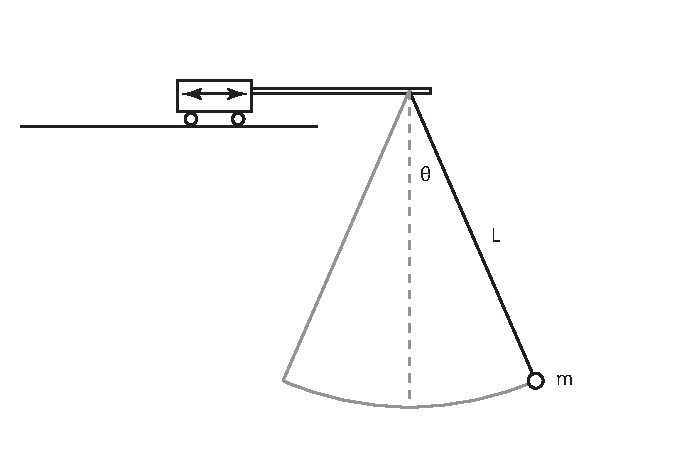
\includegraphics[]{./pendulum_resonance}
\end{center}
\end{figure}

Begin by moving the cart back and forth very slowly. What happens to the pendulum? Gradually increase the driving frequency of the cart and pay attention to what happens. Once the amplitude of the pendulum's oscillations appears to have reached a maximum, determine the frequency with which you are moving the cart back and forth. Repeat, but begin by moving the cart back and forth very quickly. What happens to pendulum? At what frequency does the pendulum appear to resonate? Do you get the same result for both cases? In other words, how many resonant frequencies does the pendulum have? How do your results compare to independent measurements of the natural frequency of the pendulum?




\end{document}
